% INTRODUCCIÓN

\cleardoublepage

\chapter{Estrategias de chunkerización para LLMs}
\label{Estrategias de chunkerización}

\section{Introducción}
La chunkerización en el ámbito de los modelos de lenguaje de gran escala (LLM) se refiere al proceso de dividir textos extensos en segmentos más manejables, conocidos como \textit{chunks}. Esta técnica es fundamental para mejorar la gestión y el procesamiento de grandes volúmenes de información en aplicaciones de inteligencia artificial que utilizan modelos de lenguaje para entender y generar texto humano.

\textbf{Necesidad de la Chunkerización:} Los modelos de lenguaje, son inherentemente limitados por la cantidad de texto que pueden procesar en una sola instancia debido a restricciones de memoria y capacidad de cálculo. Al descomponer los textos en chunks más pequeños, se facilita que el modelo maneje datos extensos de manera eficiente, permitiendo una evaluación más rápida y precisa.

\textbf{Objetivos de la Chunkerización:} El principal objetivo de la chunkerización es maximizar la relevancia y la precisión del texto procesado. Al dividir el contenido en partes significativas y manejables, se busca preservar la coherencia semántica sin sobrecargar el modelo. Además, esta estrategia es crucial para la indexación efectiva de contenidos en bases de datos vectoriales, lo que mejora la recuperación y relevancia de los resultados en consultas específicas.

\textbf{Retos de la Chunkerización:} A pesar de sus beneficios, la chunkerización presenta varios desafíos. El más significativo es determinar el tamaño óptimo de cada chunk. Si los chunks son demasiado pequeños, pueden perder contexto necesario para una comprensión completa; si son demasiado grandes, pueden exceder las capacidades de procesamiento del modelo y diluir la relevancia del contenido. Otro reto es la selección de los puntos de corte dentro del texto, que debe hacerse de manera que se preserve la integridad del contenido semántico.

La chunkerización es un proceso esencial que requiere un cuidadoso equilibrio entre tamaño de chunk, preservación del contexto y capacidades del modelo. En las siguientes secciones, exploraremos diferentes estrategias y métodos de chunkerización, evaluando sus ventajas y limitaciones en diversos contextos de aplicación.

\section{Consideraciones sobre la Chunkerización}

Al desarrollar una estrategia de chunkerización eficaz, es crucial considerar varios aspectos que influirán en el rendimiento y la eficacia del modelo de lenguaje. A continuación, se detallan algunas de las consideraciones más importantes:

\subsection{Naturaleza del Contenido}
El tipo de contenido que se está indexando es determinante en la selección de la estrategia de chunkerización. Por ejemplo, documentos largos como artículos o libros pueden requerir un enfoque diferente en comparación con contenidos más breves como tuits o mensajes instantáneos. Esta distinción afecta tanto la elección del modelo para crear los embeddings como la estrategia de chunkerización a aplicar.

\subsection{Modelo y Tamaño Óptimo del Chunk}
Dependiendo del modelo utilizado para crear los embeddings, existirán tamaños de chunk en los que el modelo desempeñará mejor. Por ejemplo, algunos modelos están optimizados para trabajar con frases individuales, mientras que otros pueden manejar mejor segmentos de texto más largos. Identificar el tamaño de chunk que maximiza la calidad de los embeddings es crucial para el éxito de la estrategia de chunkerización.

\subsection{Complejidad y Longitud de las Consultas de Usuario}
Las expectativas sobre la longitud y complejidad de las consultas de los usuarios deben guiar la manera en que se chunkeriza el contenido. Si las consultas suelen ser cortas y específicas, es posible que se prefiera chunkerizar el contenido en segmentos más pequeños para reflejar esta especificidad. En cambio, consultas más largas y complejas podrían beneficiarse de chunks más grandes que proporcionen un contexto más amplio.

\subsection{Uso de los Resultados Recuperados}
El propósito final de los chunks recuperados también juega un papel crucial. Dependiendo de si los resultados serán utilizados para búsqueda semántica, respuesta a preguntas, resumen, o cualquier otro fin, la estrategia de chunkerización podría variar para optimizar la relevancia y utilidad de la información recuperada.

\subsection{Limitaciones Técnicas}
Las limitaciones técnicas, como el número máximo de tokens que el modelo puede procesar en una sola instancia o las restricciones de memoria, son críticas para definir el tamaño de los chunks. Estas limitaciones no solo afectan cómo se chunkeriza el contenido sino también cómo se procesa posteriormente en el modelo.

Estas consideraciones son fundamentales para desarrollar una estrategia de chunkerización que no solo sea eficiente sino también efectiva en términos de mejorar la relevancia y precisión de las respuestas del modelo.

\section{Estrategias de Chunkerización}

La chunkerización puede implementarse de diversas maneras, cada una con sus propios beneficios y desafíos. A continuación, exploramos algunas de las estrategias más comunes y cómo pueden optimizarse según diferentes necesidades y contextos.

\subsection{Chunkerización de Tamaño Fijo}

Esta estrategia consiste en dividir el texto en segmentos de un tamaño predeterminado, medido en número de tokens o carácteres. La principal ventaja de este método es su simplicidad y facilidad de implementación, ya que no requiere un análisis profundo del contenido. Sin embargo, un desafío significativo es que puede cortar frases a la mitad, perdiendo contexto o generando chunks que carecen de sentido por sí solos. Para mitigar esto, se puede optar por incluir una superposición entre los chunks, donde el final de un chunk se superpone con el inicio del siguiente, ayudando a preservar el contexto (overload).

\begin{figure}[h]
\centering
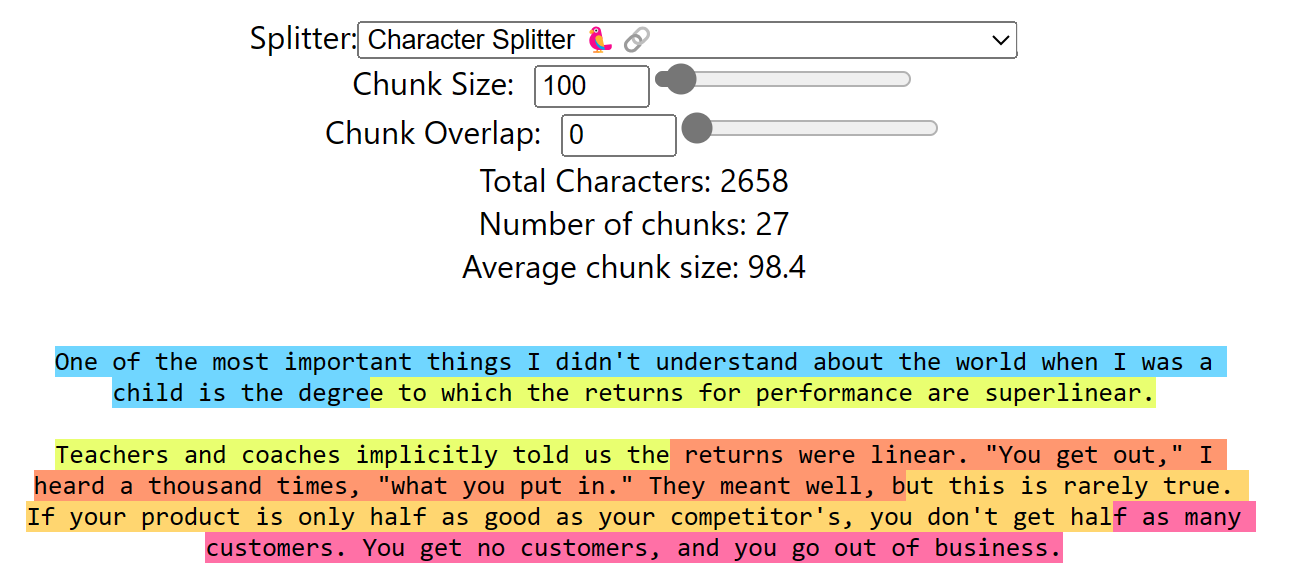
\includegraphics[width=0.8\textwidth]{figuras/capitulo4/character_splitter_100_0.png}
\caption{Ejemplo de chunkerización tamaño fijo sin overload}
\label{fig:imagen_fijo}
\end{figure}

\begin{figure}[h]
\centering
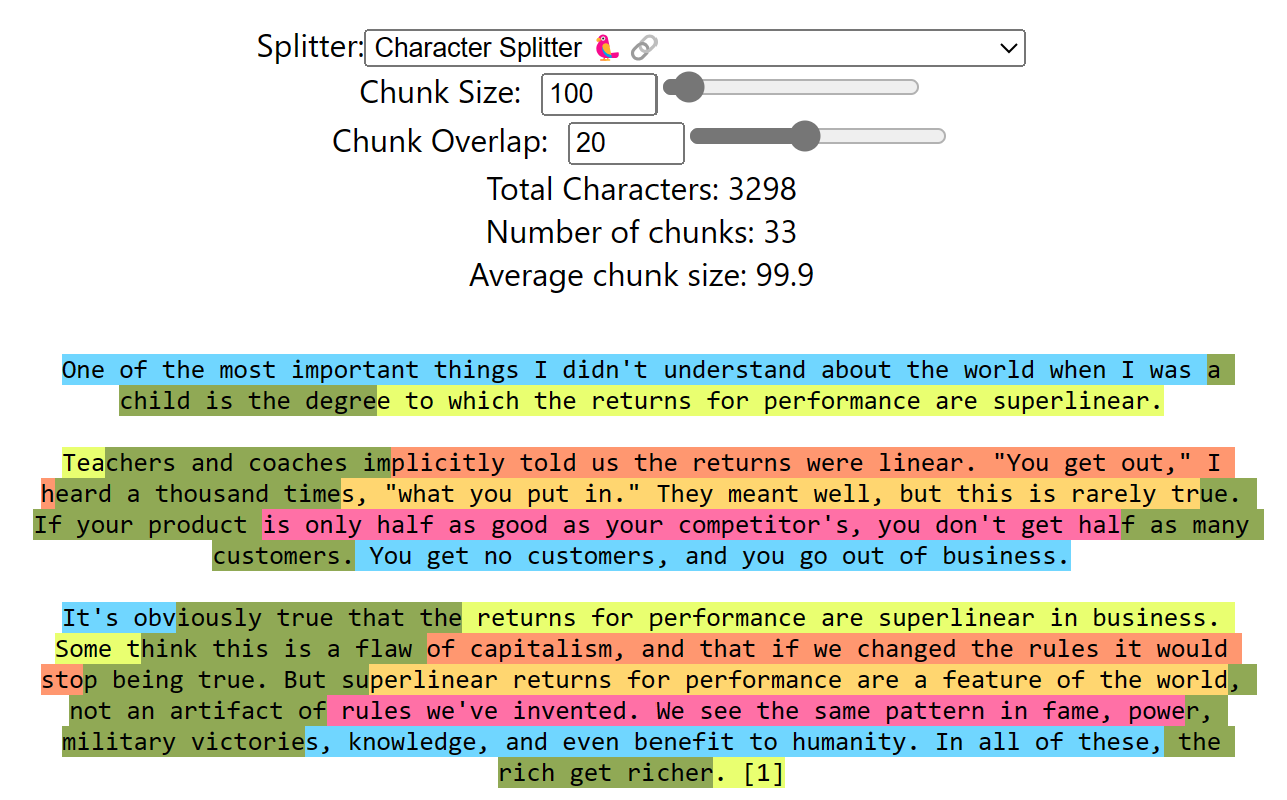
\includegraphics[width=0.8\textwidth]{figuras/capitulo4/character_splitter_100_20.png}
\caption{Ejemplo de chunkerización tamaño fijo con overload}
\label{fig:imagen_fijo_overload}
\end{figure}

\subsection{Chunkerización Consciente del Contenido}

A diferencia de la chunkerización de tamaño fijo, este método tiene en cuenta el contenido textual para determinar los puntos de corte. La chunkerización consciente del contenido puede basarse en la detección de fronteras naturales en el texto, como finales de oraciones o párrafos, asegurando que cada segmento contenga una unidad completa de información. Esto ayuda a mantener la coherencia semántica de los chunks, haciendo que cada uno sea significativo por sí mismo y mejore la calidad de las incrustaciones generadas por el modelo. Este método es particularmente útil en documentos con una estructura clara y bien definida, como artículos académicos o reportes técnicos.

\subsection{Chunkerización Recursiva}

Este enfoque implica un proceso iterativo y jerárquico de dividir el texto en chunks. Inicialmente, el texto se divide utilizando un criterio de separación amplio, y si los chunks resultantes aún son demasiado grandes o no cumplen con ciertos criterios, el proceso se repite en cada chunk hasta alcanzar el tamaño o la estructura deseada. La chunkerización recursiva es útil en textos largos y complejos donde los niveles múltiples de división permiten manejar mejor la diversidad y complejidad del contenido.

\begin{figure}[!h]
\centering
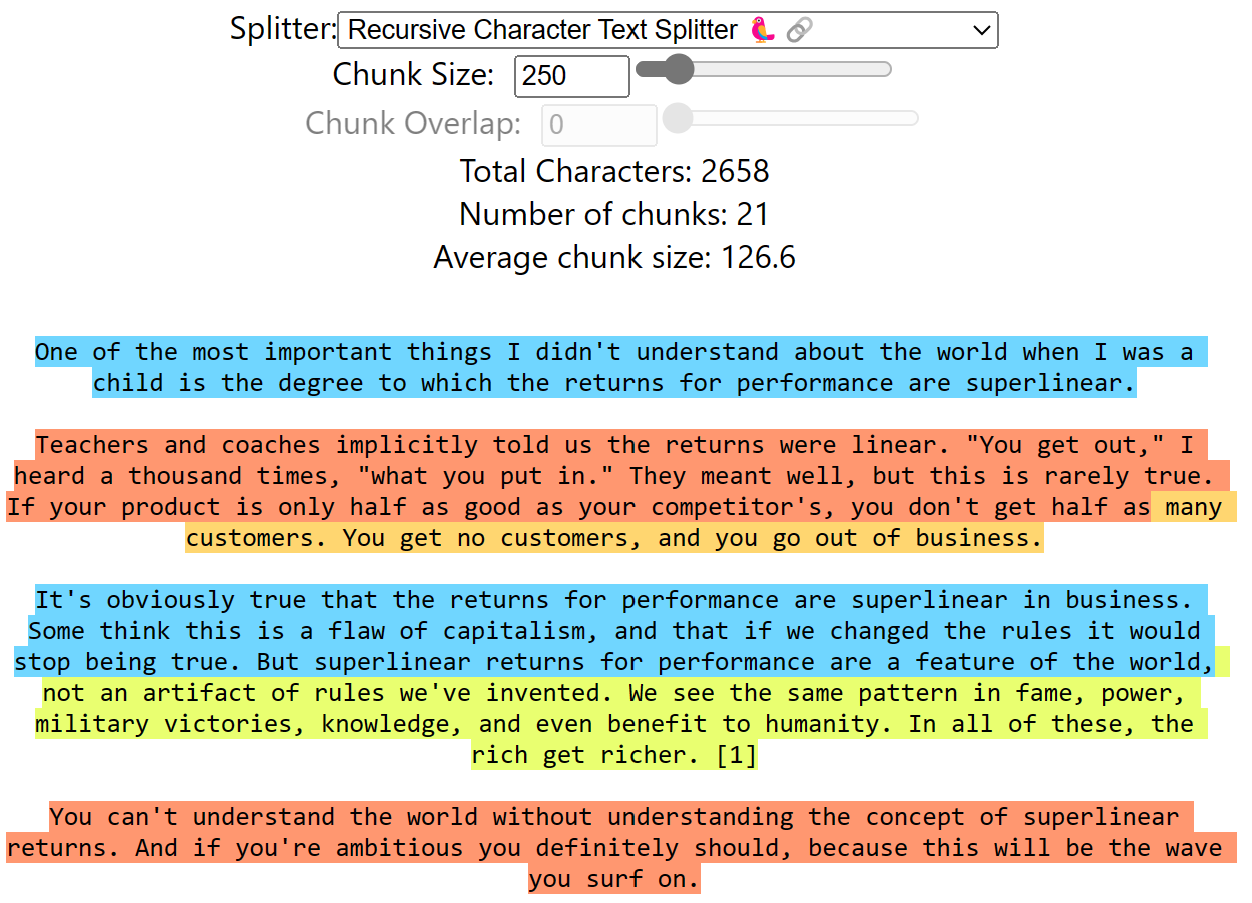
\includegraphics[width=0.8\textwidth]{figuras/capitulo4/recursive_character_splitter_250_0.png}
\caption{Ejemplo de chunkerización recursiva}
\label{fig:imagen_recursiva}
\end{figure}

\subsection{Chunkerización Especializada}

Esta estrategia se adapta a formatos de contenido específicos que requieren un tratamiento particular, como puede ser el caso de textos en Markdown o LaTeX. La chunkerización especializada reconoce y respeta la estructura y sintaxis propias de estos formatos, asegurando que los chunks resultantes conserven la integridad y funcionalidad del texto original. Por ejemplo, en un documento LaTeX, los chunks podrían definirse para encapsular secciones completas o subsecciones, preservando las etiquetas y comandos propios del formato.

Cada una de estas estrategias tiene sus propias fortalezas y puede ser más adecuada para diferentes tipos de textos y aplicaciones. La elección de una estrategia de chunkerización debe basarse en una evaluación cuidadosa de los requisitos del proyecto, la naturaleza del contenido y los objetivos específicos del sistema de procesamiento de lenguaje natural.

\begin{figure}[!h]
\centering
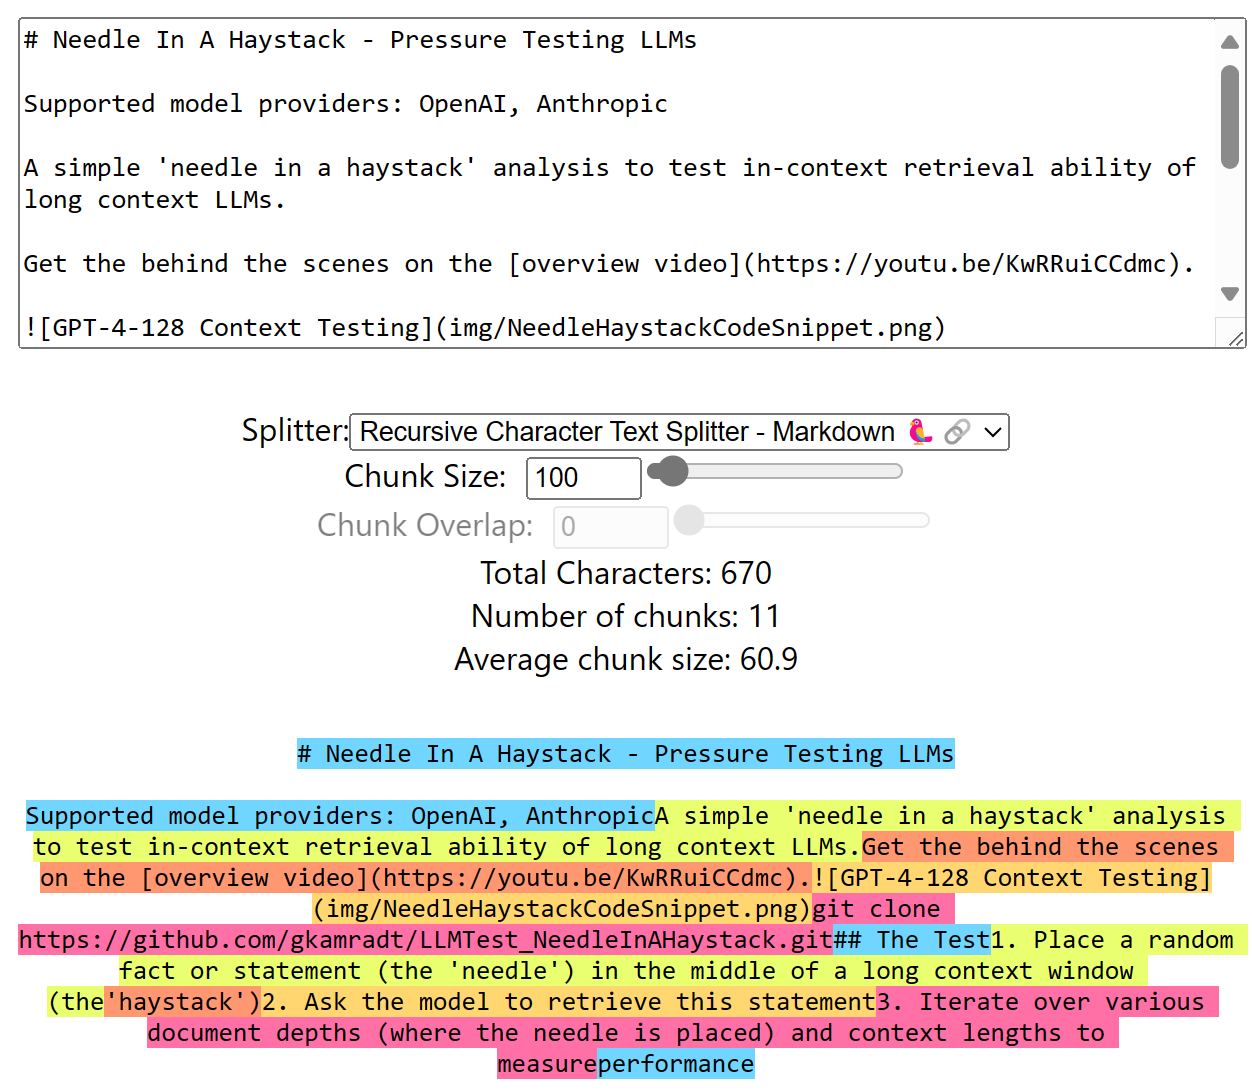
\includegraphics[width=0.8\textwidth]{figuras/capitulo4/character_md_100.png}
\caption{Ejemplo de chunkerización Especializada}
\label{fig:imagen_chunk_md}
\end{figure}

\subsection{Chunkerización Semántica}

La chunkerización semántica es una técnica avanzada que divide el texto en unidades basadas en la relevancia semántica, utilizando modelos de creación de embeddings para evaluar la similitud entre segmentos de texto.

\subsubsection{Implementación y Ventajas}
Esta estrategia se implementa mediante la transformación de texto en representaciones vectoriales y el cálculo de su similitud, agrupando segmentos similares. Es especialmente útil para mantener la coherencia del contenido en tareas de recuperación de información y análisis de texto.

\subsubsection{Desafíos y Aplicaciones}
A pesar de su efectividad, enfrenta desafíos como la alta demanda computacional y la dificultad en determinar umbrales de similitud óptimos. Su aplicación es ideal en sistemas de búsqueda semántica y en el análisis de textos complejos en contextos académicos o de investigación.

\section{Evaluación de los chunks}

La selección del tamaño de chunk adecuado es un paso fundamental para optimizar el rendimiento de los sistemas de Recuperación Aumentada por Generación (RAG). El tamaño del chunk influye directamente en la calidad de la información recuperada y, por lo tanto, en la precisión y relevancia de las respuestas generadas por el modelo. En esta sección, explicaremos los aspectos clave de la evaluación del tamaño de los chunks y cómo afecta al rendimiento de un sistema RAG utilizando LlamaIndex, una librería diseñada para optimizar este tipo de sistemas.

\subsection{Impacto del Tamaño del Chunk en el Rendimiento del Sistema}
El tamaño del chunk determina la granularidad de la información capturada durante el proceso de recuperación, lo que afecta la precisión y relevancia de las respuestas generadas. Chunk sizes pequeños, como 256 tokens, tienden a ser más detallados y contextualmente relevantes, lo que puede mejorar la alineación de las respuestas con las consultas del usuario. Sin embargo, si el chunk es demasiado pequeño, puede ocurrir que información crítica no esté contenida en los segmentos recuperados, lo que afectaría la completitud de la respuesta \citep{llamaindex-blog}.

Por otro lado, tamaños de chunks más grandes, como 512 o 1024 tokens, proporcionan un contexto más amplio pero corren el riesgo de incluir información irrelevante, lo que puede sobrecargar el sistema y disminuir la precisión de las respuestas. Este balance entre granularidad y contexto es crucial para garantizar que el sistema RAG recupere la información más relevante de manera eficiente \citep{datacamp-eval}.

\subsection{Evaluación Cuantitativa y Cualitativa del Tamaño de los Chunks}
Para determinar el tamaño óptimo del chunk, se utilizan tanto técnicas de evaluación cuantitativa como cualitativa. Las técnicas cuantitativas consisten en variar sistemáticamente el tamaño de los chunks y medir métricas como la precisión, la relevancia y la calidad de las respuestas. En experimentos típicos, se calculan métricas como el tiempo de respuesta promedio, la fe en la fidelidad de las respuestas (\textit{faithfulness}) y la relevancia (\textit{relevancy}) con respecto a las consultas \citep{vectorize-eval}. Estos datos permiten obtener medidas objetivas sobre cómo diferentes tamaños de chunks impactan en el rendimiento del sistema.

Por otro lado, la evaluación cualitativa implica la participación de jueces humanos que califican la calidad de las respuestas generadas. Factores como la coherencia, la naturalidad y la adecuación al contexto son considerados.

\subsection{Balance entre Precisión y Eficiencia Computacional}
Uno de los desafíos clave en la selección del tamaño de chunk es encontrar un equilibrio entre precisión y eficiencia computacional. Chunks más grandes pueden requerir más recursos computacionales y tiempo de procesamiento, lo que podría afectar la velocidad de respuesta del sistema, especialmente en aplicaciones en tiempo real, como chatbots o asistentes virtuales. Por el contrario, chunks más pequeños pueden ser más eficientes pero requerirán consultas de recuperación más frecuentes, lo que aumenta la sobrecarga computacional \citep{vectorize-eval}.

Este balance entre precisión y eficiencia es esencial para garantizar que el sistema RAG funcione de manera óptima dentro de las limitaciones computacionales. La selección cuidadosa del tamaño de chunk y su evaluación en función de los requisitos específicos del sistema y el dominio del problema son pasos críticos para lograr un rendimiento adecuado.\\


La evaluación del tamaño de los chunks es un proceso clave para optimizar los sistemas RAG. Mediante el uso de técnicas de evaluación cuantitativa y cualitativa, es posible determinar el tamaño óptimo que maximiza la relevancia y precisión de las respuestas, al tiempo que minimiza los costos computacionales. Adaptar el tamaño de chunk a las necesidades específicas del sistema y del dominio asegura un mejor rendimiento general del sistema \citep{llamaindex-blog,datacamp-eval}.

\section{Conclusiones}
La chunkerización es fundamental para mejorar la eficiencia y precisión en aplicaciones relacionadas con LLM. No existe una solución única para todos los casos, por lo que es crucial evaluar cada situación individualmente para encontrar la estrategia más efectiva.
